
\begin{frame}[standout]
    \Huge
    End
\end{frame}

\appendix
\backupbegin


\begin{frame}[c]% {Chromosome Conformation Technologies}
    \normalsize
    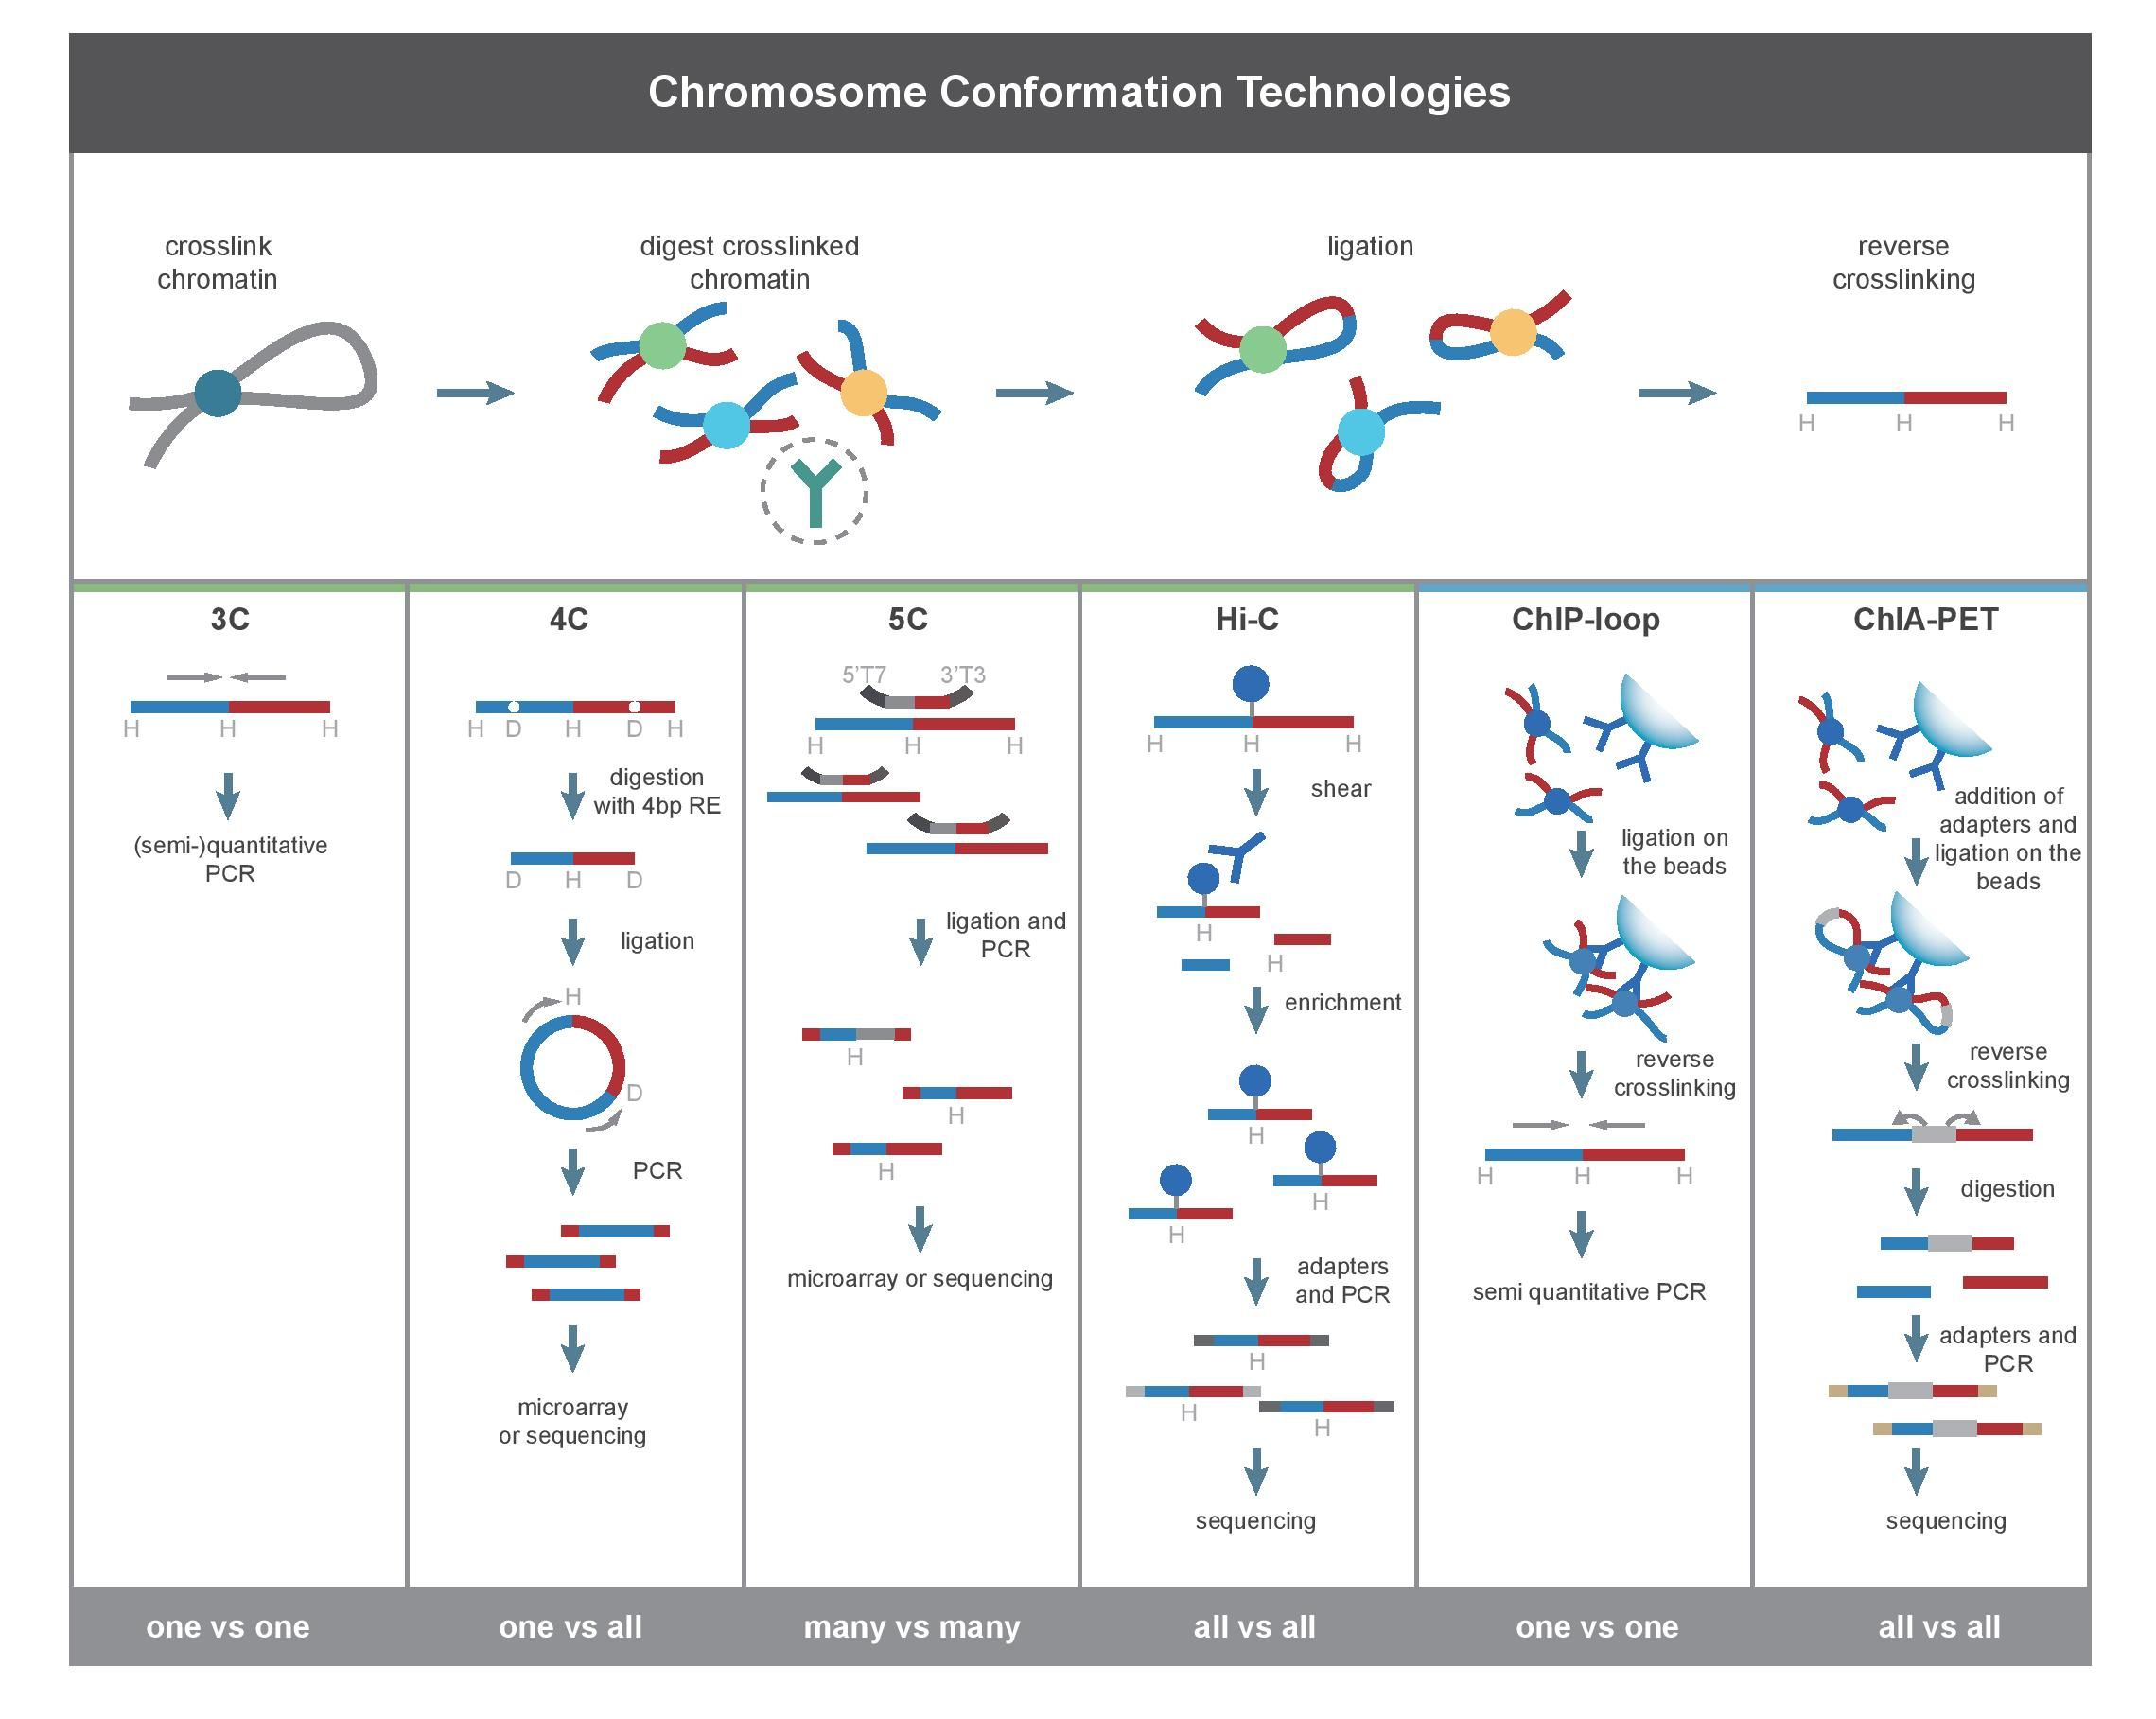
\includegraphics[scale=0.55]{Chromosome_conformation_techniques} \\
    Image from \cite{Li2014}.
\end{frame}

\begin{frame}[c]{ICE as described in Imakaev et al. 2012 \cite{imakaev2012iterative}}
    \Large
    Each iteration, compute:
    \pause
    \onslide<2->{
    \begin{equation}\label{eq:3}
        S_i = \sum_j W_{ij}
    \end{equation}
    \begin{equation}\label{eq:4}
        \Delta B_i = S_i / mean(S)
    \end{equation}
    }
    \vspace*{-\baselineskip}
    \onslide<3>{
    \begin{equation}\label{eq:5}
        W_{ij} = W_{ij} / \Delta B_i \Delta B_j
    \end{equation}
    \begin{equation}\label{eq:6}
        B_i = B_i \cdot \Delta B_i
    \end{equation}
    }
\end{frame}



\begin{frame}[c]{Rust: Code Example}
    \begin{codeboxed}{Code Example 1}
    \inputminted[linenos, fontsize=\normalsize]{Rust}{code/code_ownership.rs}
    \end{codeboxed}
\end{frame}

\begin{frame}[c]{Rust: Code Example}
    \begin{codeboxed}{Output Nr. 1}
        \footnotesize
        \verbatiminput{code/output1.txt}
    \end{codeboxed}
\end{frame}

\begin{frame}[c]{Rust: Code Example}
    \begin{codeboxed}{Code Example 2}
    \inputminted[linenos, fontsize=\normalsize]{Rust}{code/code_ownership2.rs}
    \end{codeboxed}
\end{frame}

\begin{frame}[c]{Rust: Code Example}
    \begin{codeboxed}{Output Nr. 2}
        \footnotesize
        \verbatiminput{code/output2.txt}
    \end{codeboxed}
\end{frame}


\begin{frame}[c]{Test Server Specification}
    \normalsize
    \begin{tabular}{@{}lr@{}}
        \textbf{Virtual Server Specification} & \\
        \hline
        Available Cores / Threads & 16 / 32 \\
        Working Memory (RAM) & 120 GByte \\ \\
        \textbf{Processor Specification} & \\
        \hline
        Processor & Intel® Xeon® E5-2630V4 \\
        Number of Cores/Threads & 10 / 20 \\
        Base/Turbo frequency & 2.2 GHz / 3.1 GHz \\
    \end{tabular}
\end{frame}

\backupend
